Vous pouvez rechercher n'importe quelle chanson ou artiste disponibles sur ChromaCase.
\\\\
Afin d’accéder à la page de recherche, cliquez sur le bouton recherche se trouvant sur la gauche de la page principale.

\begin{figure}[H]
	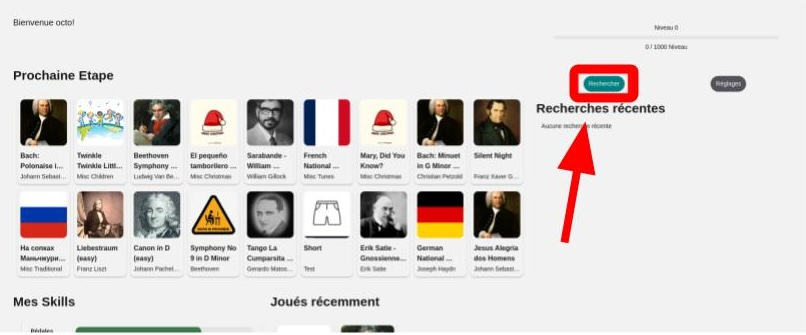
\includegraphics[width=\linewidth]{../\dir/guide/search/access-search.jpg}
	\caption{Accéder à la page de recherche}
\end{figure}
\begin{figure}[H]
	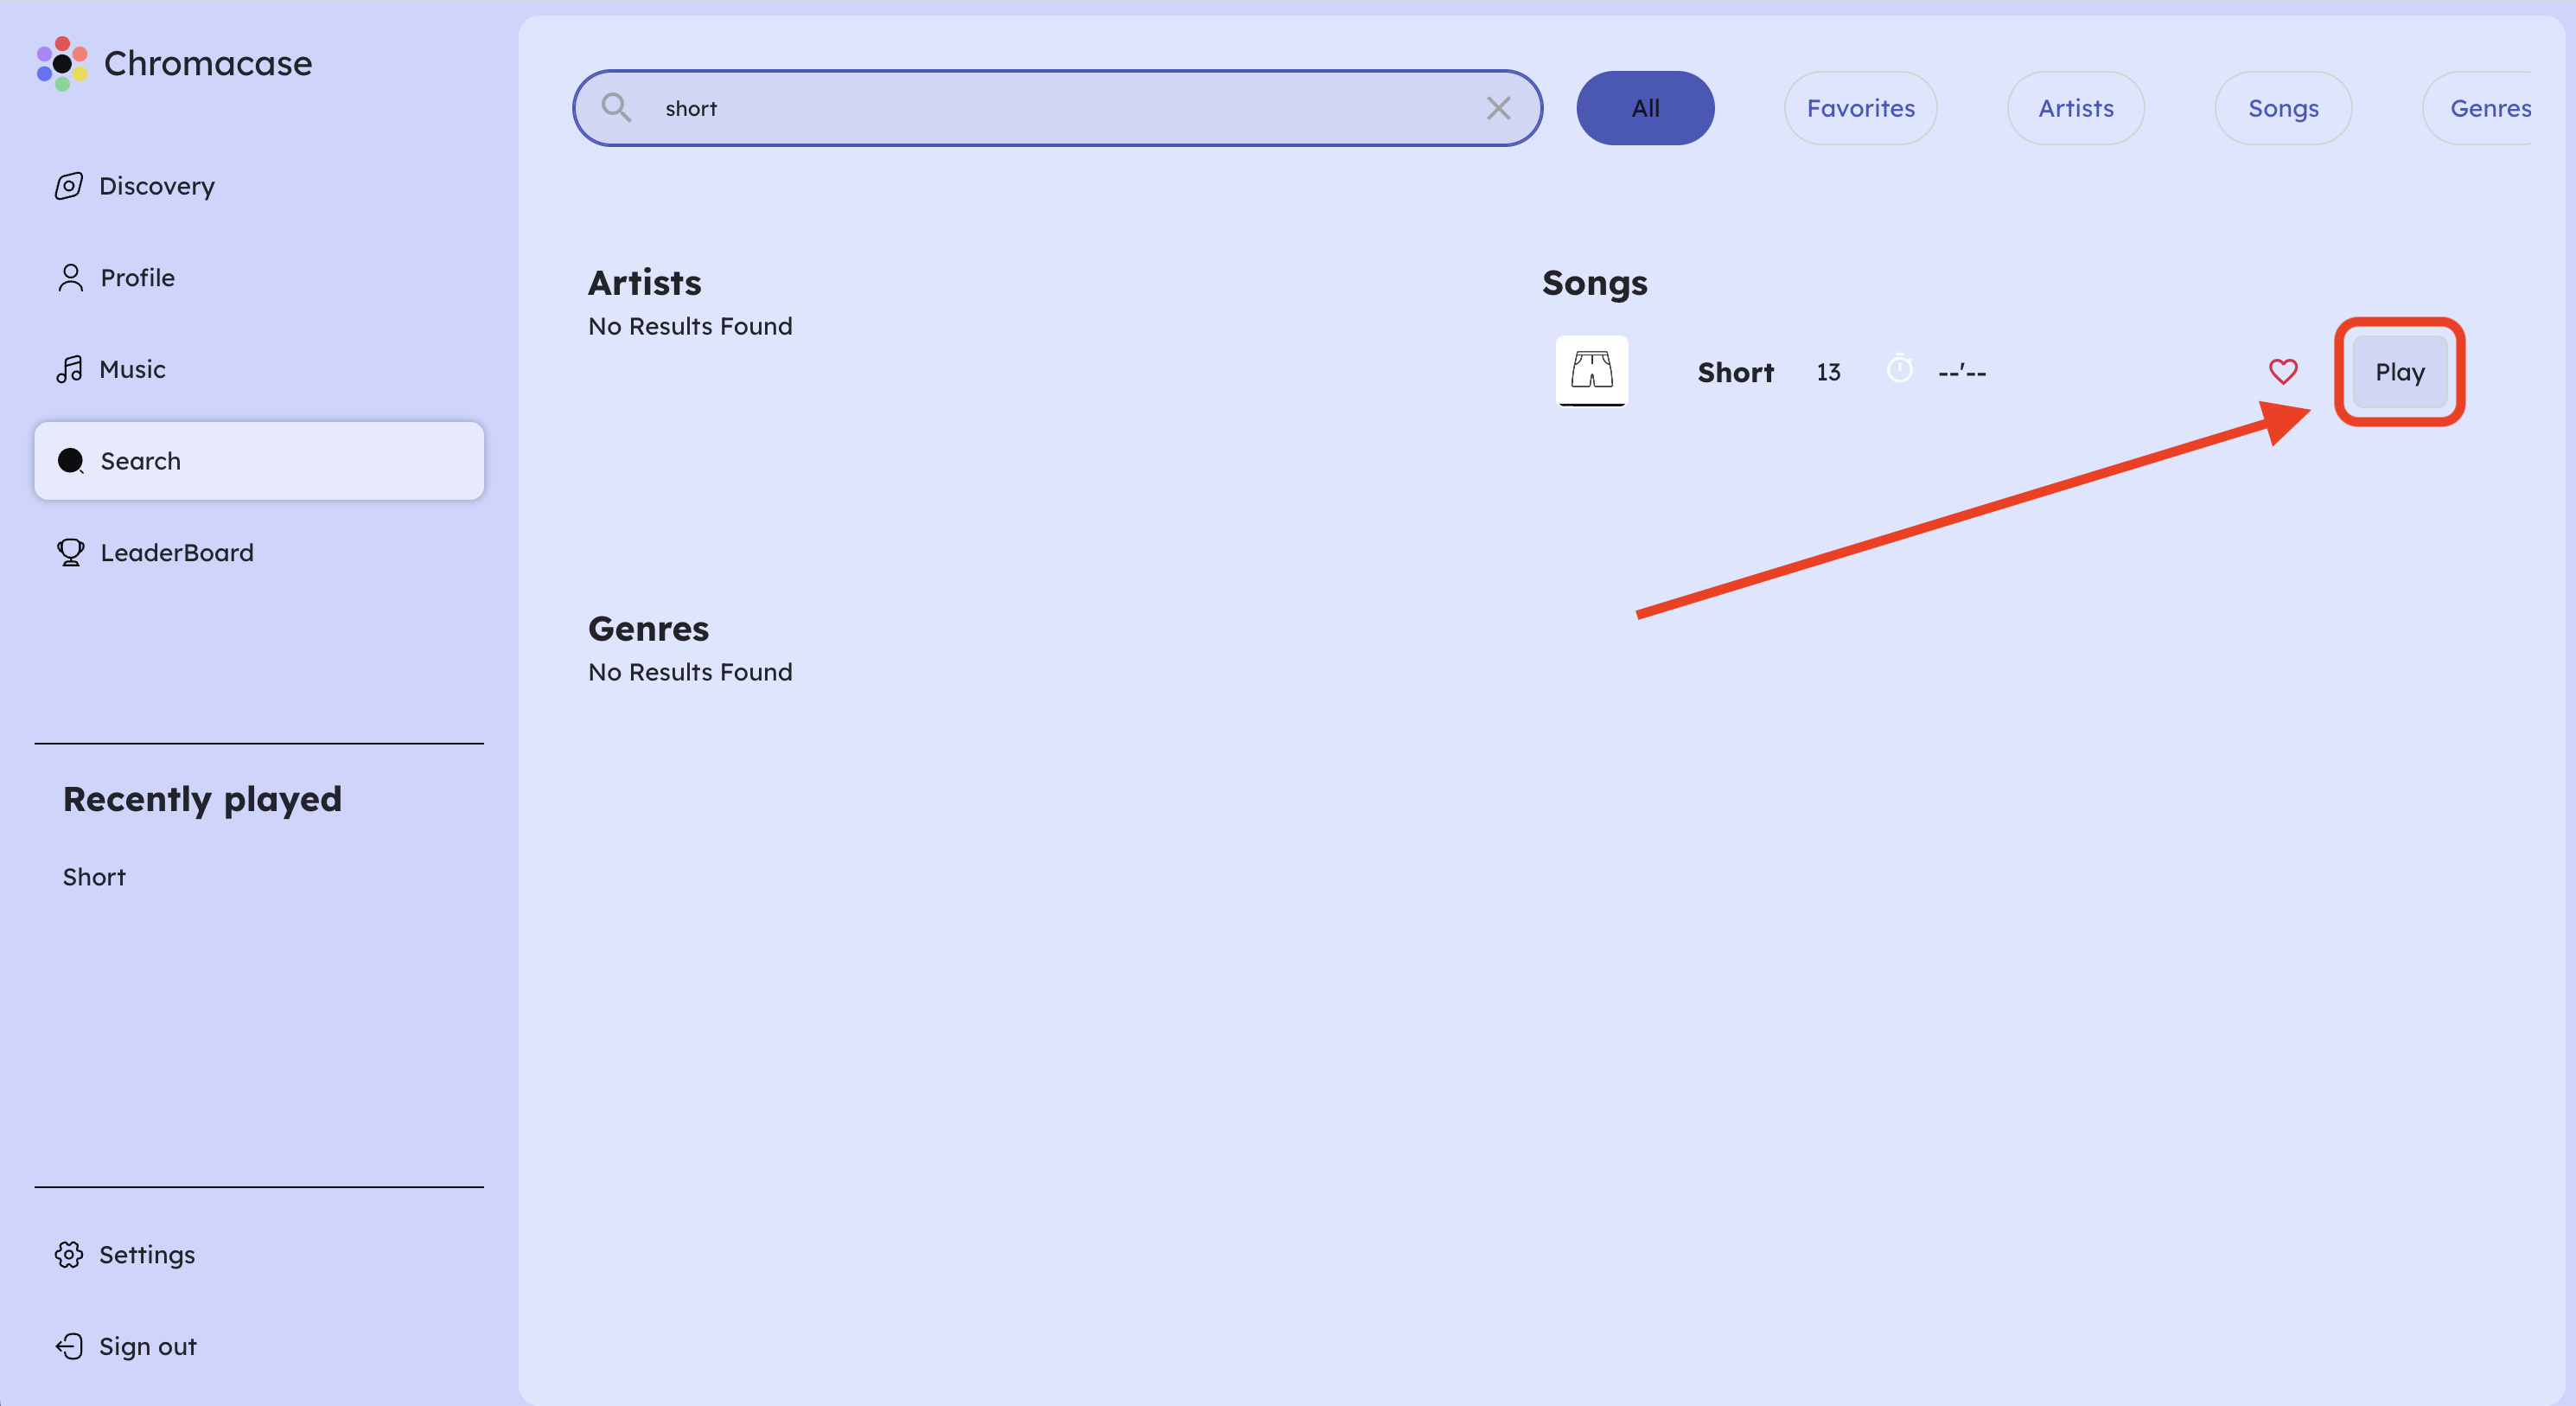
\includegraphics[width=\linewidth]{../\dir/guide/search/search.png}
	\caption{Page de recherche}
\end{figure}

\subsubsection{Rechercher une chanson}
Commencez à taper le nom de la chanson avec une catégorie compatible. Les catégories compatibles sont “Tout” et “Morceaux”.

\subsubsection{Rechercher un artiste}
Commencez à taper le nom de la chanson avec une catégorie compatible. Les catégories compatibles sont “Tout” et “Artistes”.